\documentclass[12pt,openany]{book}

\usepackage[T2A]{fontenc}            % Шрифты для кириллицы
\usepackage[russian,english]{babel}  % Пакет для поддержки русского языка
\usepackage[utf8x]{inputenc}

%%%%%%%%%% BOOK INFORMATION %%%%%%%%%%
\newcommand{\authorname}{Севумян Артем}
\newcommand{\group}{ФН11-52Б}
\newcommand{\booktitle}{Физика}
\newcommand{\subtitle}{Лабораторная работа К4}
\newcommand{\publisher}{МГТУ}
\newcommand{\editionyear}{2024}
\title{\booktitle}
\author{\authorname}

\usepackage{../latex/misc/preamble}
\graphicspath{ {../latex/images/K4.2} }

\begin{document}

\pagestyle{empty}

% Title page
\begin{titlepage}
	\centering
	
	~
	
	\vspace{24pt}
	{\scshape\Huge \booktitle\par}
	\vspace{6pt}
	{\scshape\large \subtitle\par}
	\vspace{\stretch{1.25}}
	{\itshape\large \par}
	\vspace{6pt}
	{\itshape\Large \authorname\par}
    \vspace{6pt}
	{\itshape\normalsize \group\par}
	\vspace{\stretch{6}}
	{\large \publisher\par}
\end{titlepage}


\chapter*{Задание 1}

\subsection*{1.1 Построение вольт-амперных характеристик (ВАХ)}

\vspace{10pt}

\noindent Для каждого набора данных построим по два графика.\\\\
Первый - с аппроксимацией сплайном со сглаживанием 
или же полиномом, в зависимости от ситуации.\\\\
Второй - с аппроксимацией сплайном без сглаживания и без точек с 
большими значениями положительного тока, для нахождения запирающего
напряжения.

\newpage

\noindent График зависимости тока I от напряжения U для нормальной интенсивности, 
прямой полярности и желтого фильтра (далее НПЖ).\\\\
$\text{U} = [0, 3, 6, 9, 12, 15, 18, 21, 24, 27, 30]$\\\\
$\text{I} = [0.03, 11.1, 14.5, 16.5, 17.5, 17.9, 18.4, 18.8, 19.0, 19.3, 19.5]$

\begin{center}
    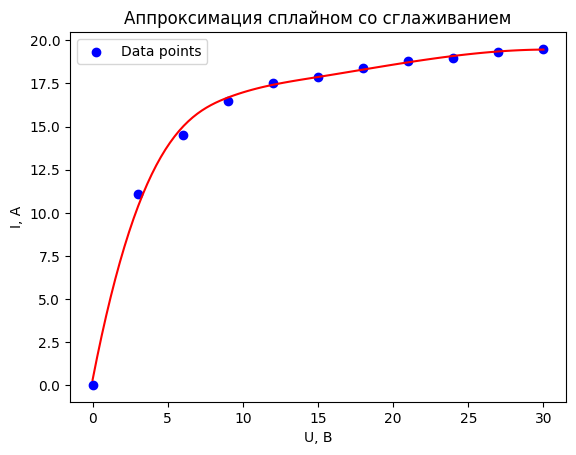
\includegraphics[scale=0.59]{1} \\

    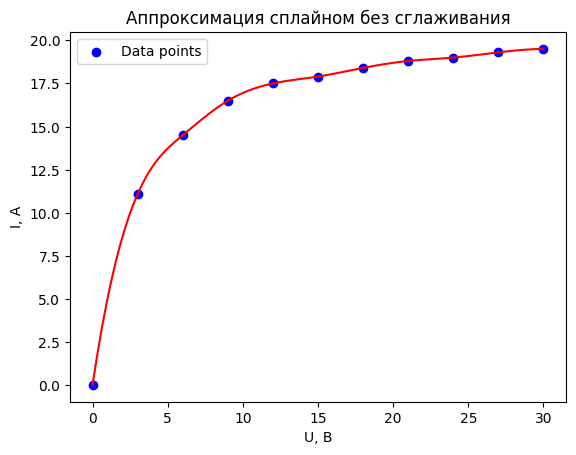
\includegraphics[scale=0.59]{2} \\
\end{center}

\newpage

\noindent График зависимости тока I от напряжения U для нормальной интенсивности, 
обратной полярности и желтого фильтра (далее НОЖ).\\\\
$\text{U} = [0.1, 0.2, 0.3, 0.4, 0.5, 0.6, 0.7, 0.8, 0.9, 1.0, 2.0, 3.0, 4.0, 5.0]$\\\\
$\text{I} = [30.8, 16.5, 8.6, 3.1, 0.6, -0.1, -0.3, -0.4, -0.5,$\\
$ -0.5, -0.6, -0.6, -0.7, -0.7]$\\
\begin{center}
    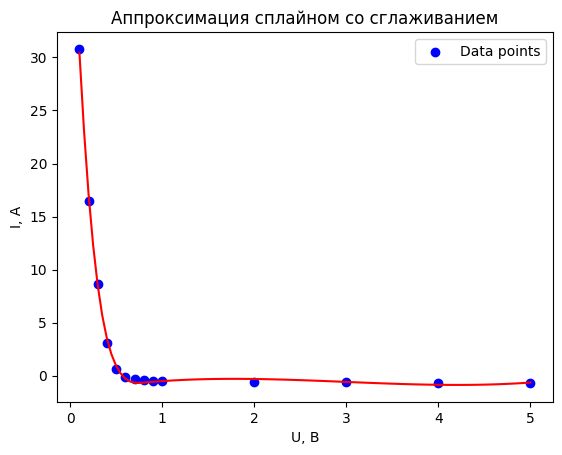
\includegraphics[scale=0.59]{3} \\

    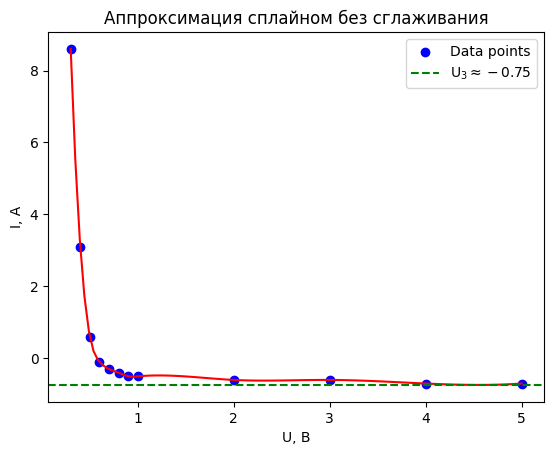
\includegraphics[scale=0.59]{4} \\
\end{center}

\newpage

\noindent График зависимости тока I от напряжения U для нормальной интенсивности, 
обратной полярности и голубого фильтра (далее НОГ).\\\\
$\text{U} = [0.5, 0.7, 0.9, 1.1, 1.3, 1.5, 1.7, 1.9, 2.1, 2.5, 3.0, 3.5, 4.0, 4.5, 5.0]$\\\\
$\text{I} = [7.4, 1.8, -0.8, -1.8, -2.1, -2.3, -2.3, -2.4, -2.4, -2.5, -2.5, -2.5,$
$-2.5, -2.6, -2.6]$\\ 

\begin{center}
    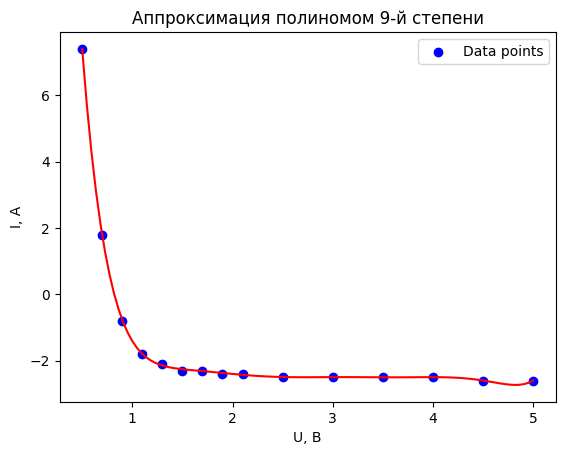
\includegraphics[scale=0.59]{5} \\

    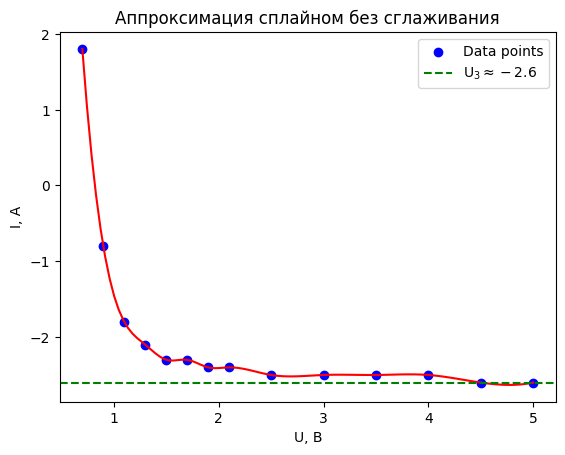
\includegraphics[scale=0.59]{6} \\
\end{center}

\newpage

\noindent График зависимости тока I от напряжения U для нормальной интенсивности, 
обратной полярности и без фильтра (далее НОБ).\\\\
$\text{U} = [1, 1.3, 1.6, 1.9, 2.2, 2.5, 2.8, 3.1, 3.4, 4.0, 4.5, 5]$\\\\
$\text{I} = [15.8, 7.9, 1.9, -1.8, -4.4, -5.5, -5.9, -6.0, -6.1, -6.2, -6.3, -6.4]$\\

\begin{center}
    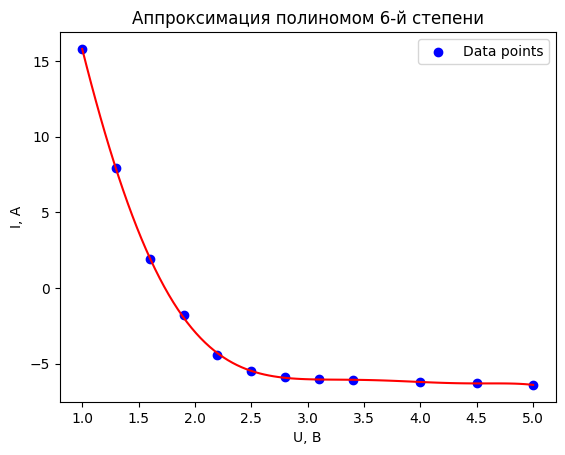
\includegraphics[scale=0.59]{7} \\

    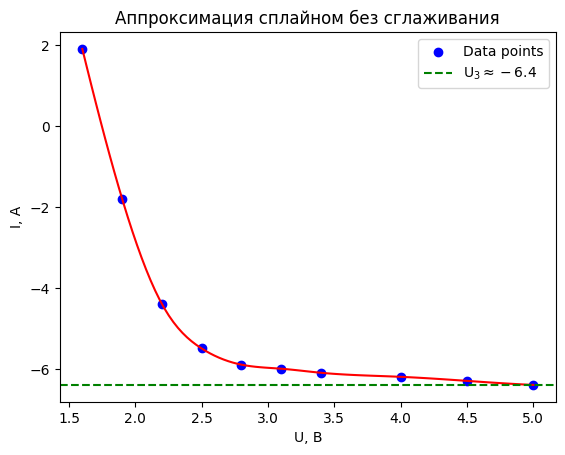
\includegraphics[scale=0.59]{8} \\
\end{center}

\newpage

\noindent График зависимости тока I от напряжения U для уменьшенной интенсивности, 
обратной полярности и желтого фильтра (далее УОЖ).\\\\
$\text{U} = [0.1, 0.2, 0.3, 0.4, 0.5, 0.6, 0.7, 0.8, 0.9, 1.0, 2.0, 3.0, 4.0, 5.0]$\\\\
$\text{I} = [3.1, 1.4, 0.4, 0, 0, -0.1, -0.1, -0.1, -0.1, -0.1, -0.1,$
$-0.1, -0.1, -0.1]$\\

\begin{center}
    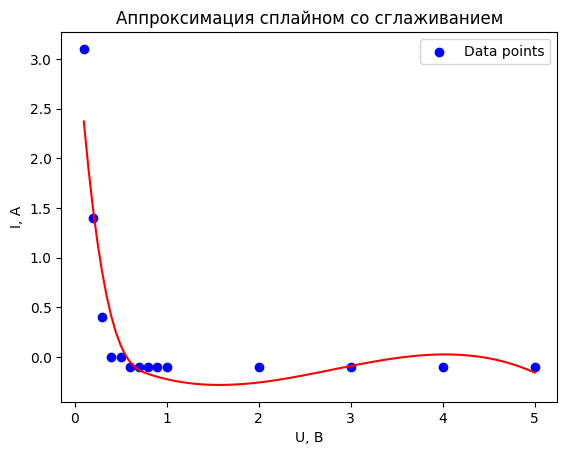
\includegraphics[scale=0.59]{9} \\

    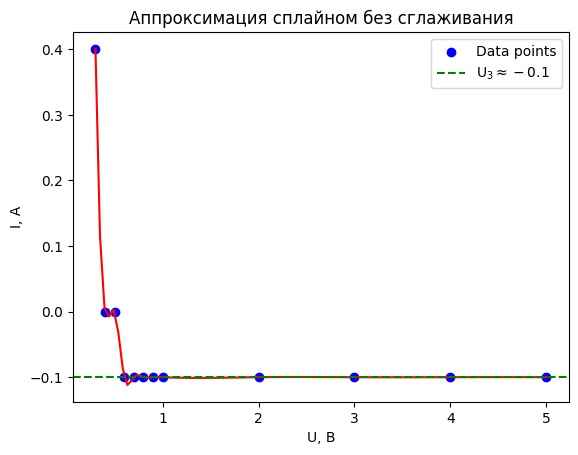
\includegraphics[scale=0.59]{10} \\
\end{center}

\newpage

\subsection*{1.2 Определение запирающего напряжения $\text{U}_\text{Z}$}

\vspace{10pt}

\noindent Из нарисованных ранее графиков извлечем найденные значения
запирающего напряжения:\\\\

\begin{center}
    \begin{tabular}{|c|c|c|c|c|}
        \hline
        & НОЖ & НОГ & НОБ & УОЖ \\
        \hline
        $\text{U}_\text{Z}$ & -0.75 & -2.6 & -6.4 & -0.1 \\
        \hline
    \end{tabular}
\end{center}

\chapter*{Задание 2}

\subsection*{2.1  Анализ зависимости $\text{U}_\text{Z}$ от частоты света}

\vspace{10pt}

\noindent На основе данных для различных фильтров и 
частот света построим график зависимости запирающего напряжения 
$\text{U}_\text{Z}$ от частоты света $\nu$. 
Частота света зависит от светофильтров:\\

{
    \begin{itemize}[noitemsep]
        \item Желтый фильтр: $\nu_1 = 5.5 \cdot 10^{14} \text{Гц}$
        \item Синий фильтр: $\nu_2 = 9.6 \cdot 10^{14} \text{Гц}$
        \item Без фильтра: $\nu_3 = 11.8 \cdot 10^{14} \text{Гц}$
    \end{itemize}
}

\vspace{2pt}

\begin{center}
    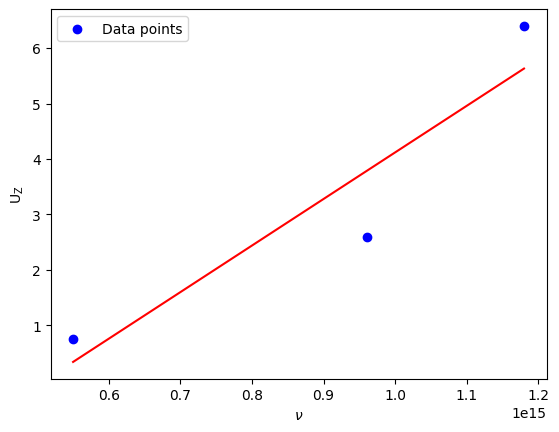
\includegraphics[scale=0.59]{11.1} \\
\end{center}

\subsection*{2.2  Определение постоянной Планка}

\vspace{10pt}

\noindent По наклону прямой на графике зависимости $\text{U}_\text{Z}$ 
от $\nu$ определим постоянную Планка h по формуле:\\

\begin{equation*}
    \text{h} = \text{e} \cdot \cfrac{\Delta \text{U}_\text{Z}}{\Delta \nu}
\end{equation*}

\begin{center}
    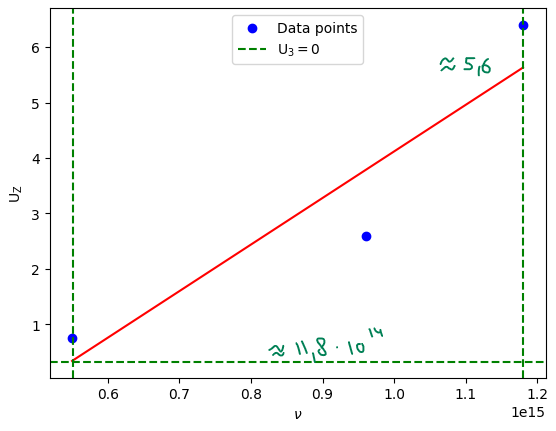
\includegraphics[scale=0.59]{11.2} \\
\end{center}

\begin{equation*}
    \text{h} \approx 7.6 \cdot 10^{-34}
\end{equation*}

\vspace{10pt}

\noindent (С 2019 года значение постоянной Планка считается 
зафиксированным и точно равным величине $\text{h} = 6.626070
15 \cdot 10^{-34} \text{кг} \cdot \text{м}^2 \cdot \text{с}^{-1}
(\text{Дж} \cdot \text{c})$)

\subsection*{2.3  Определение работы выхода A и красной границы фотоэффекта}

\vspace{10pt}

\noindent По пересечению графика с осью абсцисс (где $\text{U}_\text{Z}$) 
определим красную границу фотоэффекта $\nu_0$ и работу выхода A, 
используя соотношение:

\begin{equation*}
    \text{A} = \text{h} \cdot \nu_0
\end{equation*}

\vspace{10pt}

\noindent значение $\nu_0 \approx 550659604190919.2$, следовательно

\begin{equation*}
    \text{A} = 7.6 \cdot 10^{-34} \cdot 550659604190919.2 \approx 4.18 \cdot 10^{-19}
\end{equation*}

\subsection*{2.4  Определение энергии фотонов}

\vspace{10pt}

\noindent Определим энергию фотонов для разных частот света, 
используя значение постоянной Планка, которое мы получили. 
Формула для энергии фотонов:

\begin{equation*}
    \varepsilon = \text{h} \cdot \nu
\end{equation*}

\vspace{10pt}

{
    \begin{itemize}[noitemsep]
        \item Для видимого света: $\nu_1 = 5.5 \cdot 10^{14} \text{Гц} \implies \\ \varepsilon_1 \approx 4.18 \cdot 10^{-19}$
        \item Для ультрафиолетового света: $\nu_3 = 11.8 \cdot 10^{14} \implies \\ \varepsilon_3 \approx 8.96 \cdot 10^{-19}$
    \end{itemize}
}

\subsection*{2.5  Определение потока излучения}

\vspace{10pt}

\noindent Вычислим поток излучения $\Phi$, прошедший через желтый фильтр. 
Этот поток пропорционален количеству фотонов, которые выбивают 
электроны из фотокатода, и рассчитывается по формуле:

\begin{equation*}
    \Phi = \cfrac{\text{h} \nu \text{J}_0}{\text{e} \text{Y}}, \quad \text{где}
\end{equation*}

\vspace{10pt}

{
    \begin{itemize}[noitemsep]
        \item h — постоянная Планка, которую мы вычислили ранее
        ($\text{h} = 7.6 \cdot 10^{-34}$),
        \item $\nu$ — частота излучения, соответствующая желтому фильтру 
        ($\nu_1 = 5.5 \cdot 10^{14} \text{Гц}$),
        \item J$_0$ — ток насыщения, который можно определить из 
        вольт-амперной характеристики для прямой полярности
        (J$_0$ = 19.2 $\cdot 10^{-3}$ А),
        \item e — заряд электрона (e $ = 1.6 \cdot 10^{-19} \text{Кл}$),
        \item Y — квантовый выход фотокатода, который мы 
        возьмем из паспорта лабораторной установки (Y = 0.1).
    \end{itemize}
}

\begin{equation*}
    \Phi \approx 0.5012
\end{equation*}

\end{document}
